%%notwendige packages

%----------------------------

\documentclass[12pt]{article}
%benötigt man immer
\usepackage{amsmath}
%is used for numbering of equations
\usepackage[english]{babel}
\usepackage[utf8x]{inputenc}
\usepackage{varwidth}
\usepackage{float}
% Table caption on top of tables
\floatstyle{plaintop}
\restylefloat{table}
%----
\usepackage{makecell}
\usepackage{enumitem}

% allows index generation
\usepackage{makeidx}
\makeindex

% equation, table and figure numbering should start with section number e.g. (3.1)
\numberwithin{equation}{section}
\numberwithin{table}{section}
\numberwithin{figure}{section}

%fonts
\usepackage[T1]{fontenc}
\usepackage{textcomp}
\usepackage{mathptmx}
\usepackage{tabularx}
\usepackage{multirow}
\usepackage{enumitem}
%small fonts for captions of figures and tables
\usepackage{caption}
\captionsetup[figure]{font = footnotesize}
\captionsetup[table]{font = footnotesize}


%format
% Witwen und Waisenkinder vermeiden
\clubpenalty=4500	% Waisen vermeiden (erste Zeile eines neuen Absatzes als letzte Zeile einer Seite)
\widowpenalty=10000	% keine Witwen zulassen (letzte Zeile eines Absatzes am Beginn einer neuen Seite)

% Seitenraender einstellen
\usepackage{geometry}
\geometry{a4paper,left=30mm,right=20mm, top=20mm, bottom=20mm}

% Zeilenabstand
\linespread{1.5} 

%Graphics
\usepackage[final]{graphicx} 	
\usepackage[twoside,figuresright]{rotating}
\usepackage{subcaption} 
%\usepackage{subfigure} 

% Adjust tables (and figures) to textwidth...
\usepackage{adjustbox}

%For tables, to color whole row without missing pieces...
\usepackage{tabularx}
%\usepackage[table]{xcolor}  % option loads »colortbl«

% Initialize Makro for table heads
\renewcommand\theadfont{\bfseries\sffamily}

% Highlighting rows, columns and headers of tables
\usepackage{color, colortbl}
\definecolor{Gray}{gray}{0.9}
\definecolor{LightCyan}{rgb}{0.88,1,1}
\definecolor{SeaBlue}{rgb}{0.3, 0.58, 1}

%acronym package for Abbreviations
\usepackage{acronym}

%Create Statutory Declaration page for signatures
\newcommand{\namesigdate}[2][3cm]{%
  \begin{tabular}{@{}p{#1}@{}}
    #2 \\[2\normalbaselineskip] \hrule \\[0pt]
    {\small \textit{Signature}}
  \end{tabular}
}

%----------------------------

\begin{document}

\thispagestyle{empty}	
% !TEX root = Master.tex

%titlepage
\thispagestyle{empty}
\begin{center}


\begin{minipage}{0.75\linewidth}
    \centering
%University logo
    
\includegraphics[scale = 0.7]{figures/uni_goettingen_logo.pdf}\\
    
    %\rule{0.4\linewidth}{0.15\linewidth}\par
    \vspace{1cm}
    
% Master Thesis
{{\Huge \textbf{Master Thesis} \par}}
    
\vspace{0.5cm}
    
%Thesis title
    {{\LARGE Multivariate modelling of the dependency structure between article sales of a sportswear manufacturer\par}}
    \vspace{1cm}
    
    
%Author's name
\begin{center}
Author\\
{\LARGE \textbf{Petros Christanas}} \\


\vspace{0.5cm}

Matriculation Number \\
{\large 11604278}

\vspace{1cm}

{\Large Student of Applied Statistics M.Sc.}\\
{\large Chair of Statistics and Econometrics}

\end{center}
    
    \end{minipage}
\end{center}


\vspace{2cm}

\noindent Supervisors\\
\noindent {\Large \textbf{Prof. Dr. Thomas Kneib}} \\
\noindent {\Large \textbf{Der andere}} \\

\vspace{1cm}
    
%Date
\begin{flushleft}
\noindent {\Large \today}
\end{flushleft}

    
    

\clearpage


\newpage
\null\thispagestyle{empty}
\newpage
\thispagestyle{empty}
\section*{Confidentiality Clause}
% !TEX root = Master.tex

Write in here the text for the confidentiality clause!

%\clearpage
\newpage
\null\thispagestyle{empty}
\newpage
\thispagestyle{empty}
\section*{Statutory Declaration}
% !TEX root = Master.tex

\vspace{2cm}

I hereby declare that I wrote this thesis paper
independently, without assistance from external parties, and without use of other resources than
those indicated. All information taken from other publications or sources in text or in meaning
are duly acknowledged in the text. The written and electronic forms of the thesis paper are the
same. I give my consent to have this thesis checked by plagiarism software.

\vspace{5cm}

Nuremberg, \today


\vspace{2cm}


\noindent\begin{tabular}{ll}
\makebox[2.5in]{\hrulefill} \\
Petros Christanas \\
\end{tabular}




\newpage
\null\thispagestyle{empty}
\newpage
\thispagestyle{empty}
\section*{Acknowledgments}
% !TEX root = Master.tex

\vspace{3cm}



I would like express my deepest gratitude towards Dr. Alexander März, who guided me throughout this thesis with his expertise and is always finding the time to help during this special times. I would also like to thank the entire adidas Data Science \& AI team for contributing a great deal to my learning journey and giving me the opportunity to conduct this thesis.\\
I am also sincerely grateful towards Prof. Dr. Thomas Kneib for supervising my Master thesis and moreover for leading the study program of Applied Statistics and passing on his knowledge to his students in the best way possible.\\
Last but not least, I would like to thank my fellow students Patrick Neff and Malte Lehna who were playing a key role in my personal growth and with whom I had an unforgettable time in Göttingen. 

\vspace{1.5cm}


\textbf{\textgreekfont{Ευχαριστώ θερμά τους γονείς μου για την άνευ όρων υποστήριξη. Σας αγαπώ!}}



\newpage
\null\thispagestyle{empty}
\newpage


	
%\pagenumbering{Roman} 	
\thispagestyle{empty}
\tableofcontents
\newpage




\newpage

\pagenumbering{arabic} 
\setcounter{page}{1} 

\section{Introduction}
% !TEX root = Master.tex


Write in general something like an "abstract", what is the pipeline of the thesis as a whole..

Quick test for user specified compiling and citing:\\
\cite{lutkepohl1996specification}\\
\citep{Rcoreteam}\\
\cite{Rcoreteam}\\




\clearpage
\section{Study Area \& Data Sources}
\subsection{Forest Classification}
% !TEX root = Master.tex

The study area is a private forest enterprise in Gartow (Niedersachsen) Germany. It measures around 5674.2 ha in total (see Table \ref{tab:sizes}) and is a relatively homogenous forest consisting mostly of pine trees.

\begin{table}[H]
\setlength\arrayrulewidth{1pt}  
\centering
\begin{tabular}{|c |c |c |c|}
\hline 
\rowcolor{Gray}
\textbf{Stratum} & \textbf{Location Class} & \textbf{Area [ha]} & \textbf{Relative Area} \\ 
\hline 
1 & 1 & 338.6 & 0.06 \\ 
\hline 
2 & 2 & 1546.9 & 0.27 \\ 
\hline 
3 & 3 & 2129.3 & 0.38 \\ 
\hline 
4 & 4 & 1550.5 & 0.27 \\ 
\hline 
G & 2 & 108.9 & 0.02 \\ 
\hline 
\rowcolor{SeaBlue}
Total & - & 5674.2 & 1 \\ 
\hline 
\end{tabular} 
\caption{Size of the different stratum and associated sampling grids. Stratum 2 and G have been merged to Location Class 2 which results in an identical sampling grid.}
\label{tab:sizes}
\end{table}

The forest itself is split into stratum to take site conditions, forest structure and thus natural variation of the areas into account (see Figure \ref{fig:Gartow Map}). The assessment of variation was based on a forest inventory conducted 2008
(see Table \ref{tab:Sample_Variation}).

\begin{table}[H]
\setlength\arrayrulewidth{1pt}  
\centering
\begin{adjustbox}{max width=\textwidth}
\begin{tabular}{|c |c |c |c |c |c |c |c|}
\hline 
\rowcolor{Gray}
\textbf{Stratum} & \textbf{Location Class} & \textbf{Area [ha]} & \textbf{Relative Area} & \textbf{Sample Size} & \textbf{Mean Volume / ha} & \textbf{Sample Variance} & \textbf{SE\%} \\ 
\hline 
1 & 1 & 338.6 & 0.06 & 159 & 180.19 & 104.24 & 5.67 \\ 
\hline 
2 & 2 & 1546.9 & 0.27 & 805 & 246.75 & 22.75 & 1.93 \\ 
\hline 
3 & 3 & 2129.3 & 0.38 & 542 & 195.41 & 13.15 & 1.86 \\ 
\hline 
4 & 4 & 1550.5 & 0.27 & 134 & 131.90 & 30.45 & 4.18 \\ 
\hline 
G & 2 & 108.9 & 0.02 & 55 & 271.26 & 734.08 & 9.99 \\ 
\hline 
\rowcolor{SeaBlue}
Total & - & 5674.2 & 1 & 1659 & 196.37 & 6.46 & 1.29 \\ 
\hline 
\end{tabular} 
\end{adjustbox}
\caption{Mean volume and sample variation estimates of the forest inventory 2008. Stratum 2 and 3 show little relative standard
error (SE\%), while stratum 1 inhibits more variation. Stratum G, which covers only 2\% of the total area has a typical high variation}
\label{tab:Sample_Variation}
\end{table}

Main sources of the variation in the growing stock can be assigned by the varieties in the tree species and the age distribution of the trees. Young and therefore small trees have a smaller diameter. If an area has been cultivated around the same timespan with identical species, the trees are expected to be centred on a certain diameter. On the other hand, a very diverse area in species and time will have naturally more variation (see Figure \ref{fig:barplots_Gartow})

\begin{figure}[H]
  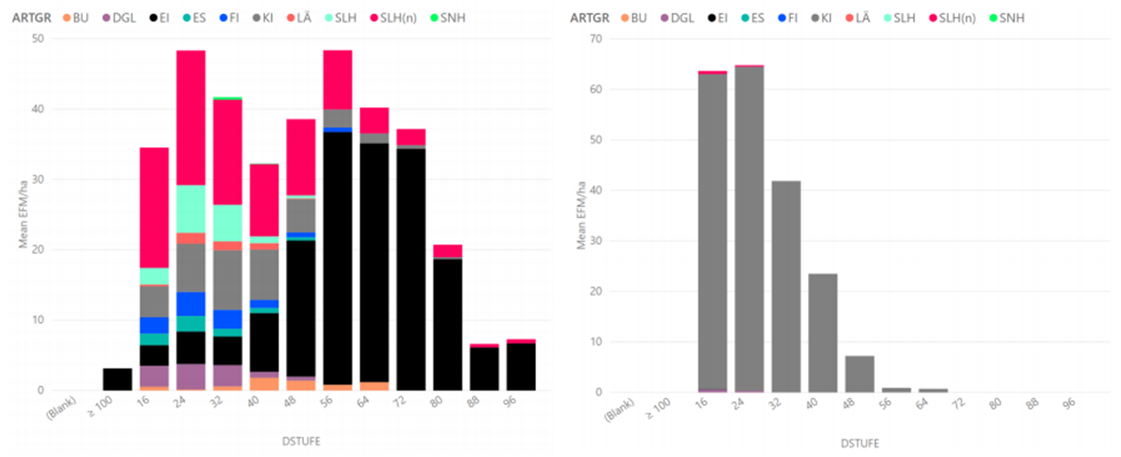
\includegraphics[width=\textwidth]{barplots_Gartow.png}
  \caption{The bar plots (left to right: stratum 1, stratum 4). The bars indicate the mean volume per ha for different diameter classes [1].}
  \label{fig:barplots_Gartow}
\end{figure}

Sampling activities are adjusting according to the inhibited variation of the stratum type (see Section \ref{Inventory Data}).

\begin{figure}[H]
  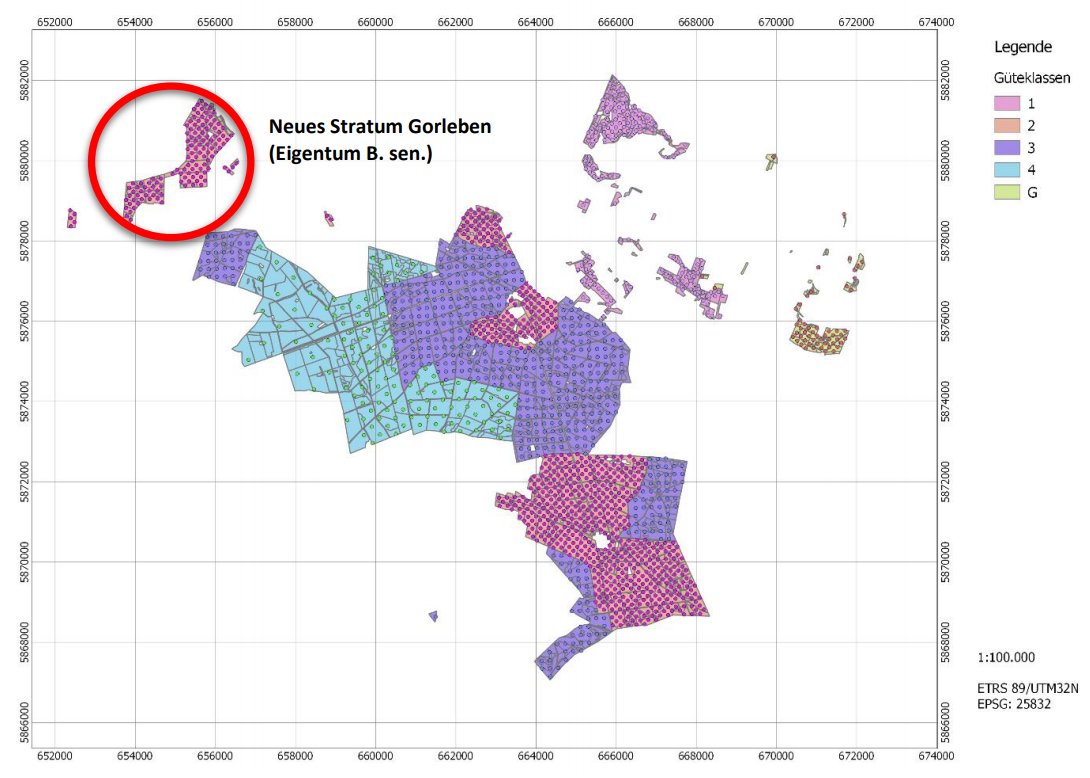
\includegraphics[width=\textwidth]{Gartow_map.png}
  \caption{The forest of Gartow is divided into stratums based on past observed variation and ownership and subdivided into compartments indicated by grey lines. Each point within a section indicate a sampling point [1].}
  \label{fig:Gartow Map}
\end{figure}

The stratum themselves are subdivided into compartments with the intention to create homogeneous sub regions (see Figure \ref{fig:Gartow Map}). The diameter distribution must be found for each of those compartments.

\subsection{Inventory Data} \label{Inventory Data}
% !TEX root = Master.tex

In spring 2018, a sample-based forest inventory was carried out in Gartow. 942 sampling locations are defined which are spread over the forest based on a stratified sampling approach. This accounts for the past observed variation within the regions. Compartments of stratum 1 and 2 are sampled with a dense sampling grid, while 3 and 4 have a wider sampling grid (see Table \ref{tab:Sample_Variation} \& Figure \ref{fig:Gartow Map}).\\

At each sampling location (so called plots) several attributes of the trees within a certain circular area are measured. The parameters of primary interest in this study are the diameter, species and height. The diameter is measured at breast height (around 1.3 meters) with a measuring tape. Subsequently, the height is measured with varying, but established methodologies. Unlike the diameter, not every tree height is collected. In each plot, three main species trees (less if there are fewer trees) are measured. To cover the total range of values, a small, a medium sized and a large one is gauged. Additionally, one tree of every other species is measured to cover the variety of species. Table \ref{tab:Measured Trees} provides an overview of total measured trees.

\begin{table}[H]
\setlength\arrayrulewidth{1pt}  
\centering
\begin{tabular}{|c| c|}
\hline 
\rowcolor{Gray}
\textbf{Stratum} & \textbf{\# Measured Trees} \\ 
\hline 
1 & 1287 \\ 
\hline 
2 & 3434 \\ 
\hline 
3 & 2734 \\ 
\hline 
4.1 & 616 \\ 
\hline 
4.2 & 792 \\ 	
\hline 
G & 523 \\ 
\hline 
GL & 619 \\ 
\hline 
\rowcolor{SeaBlue}
Total & 10005 \\ 
\hline 
\end{tabular} 
\caption{Overview of number of measured trees for height and diameter per Stratum}
\label{tab:Measured Trees}
\end{table}


\subsection{LiDAR} \label{LiDAR}
% !TEX root = Master.tex

While the previously described data will be used for modelling, data captured by the airborne LiDAR is of main interested in this report, since the ability of innovating forest inventory is discussed.\\

LiDAR uses a laser scanning system to capture distances. In context, laser scanning is referred to the active emitting and sensing of light. Thus, Light Detection and Ranging is a suitable description of the mechanics, also known as LADAR (Laser Detection and Ranging). LiDAR is a more generalized definition, as instead of laser- light also xenon or flash lamps can be used [2]. A high-level definition of the functionality of LiDAR is as follows. Laser beams are continuously emitted of the LiDAR system, mounted on an airborne vehicle. The coordinates are throughout captured by a GPS (Global Positioning System) and IMU (Inertial Measurement Unit – used to capture adjust for e.g. inclined positioning, acceleration of the vehicle). Laser or xeon/flash light is emitted of an active sensor and the distance captured once it is traveled back to the scanner. As forests have a relatively turbulent surface and only little light can reach the surface of the forest, many systems only capture the first and last impulse [3]. The cloud of captured points can then be used to create a 3-D image of the forest (see Figure \ref{fig:LiDAR}).

\begin{figure}[H]
  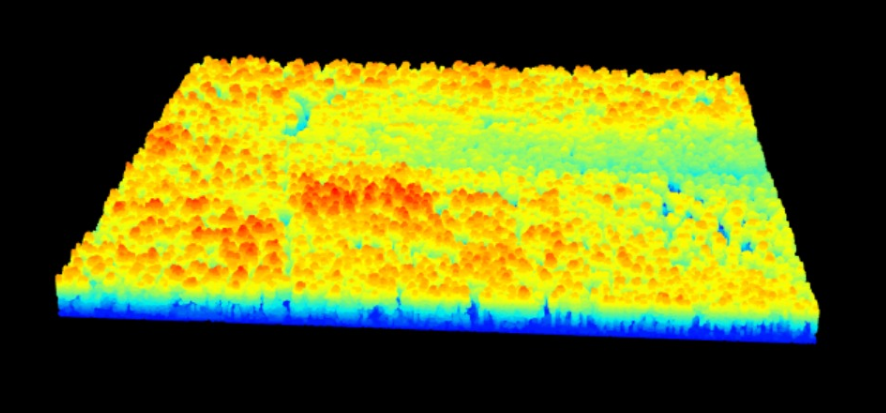
\includegraphics[width=\textwidth]{lidar.png}
  \caption{3-D Image of a small area of the forest of Gartow made by the airborne LiDAR. The determined height is colorized. A
dense group of height trees is found almost in the middle and directly behind an aisle of small trees.}
  \label{fig:LiDAR}
\end{figure}

Main benefits of LiDAR compared to other systems is the ability to capture data regardless of sun positioning, day or night and the ability to map through the highly dense areas (the canopies of the trees). The main benefit compared to the traditional way of forest inventory is relative intuitive. A plane is capable of objectively measuring the forest subject to this report in under a week; while a forester must inspect every single hectare, providing a more subjective intuition of the forest inventory.

\begin{table}[H]
\setlength\arrayrulewidth{1pt}  
\centering
\begin{adjustbox}{max width=\textwidth}
\begin{tabular}{|c|c|}
\hline
\rowcolor{Gray}
\textbf{Flight Altitude}              & \textbf{Approx. 590m above ground} \\ \hline
Nominal point density (laser)         & 6 points / m²                      \\ \hline
Ground resolution                     & 4.3cm                              \\ \hline
Point density (to circumvent overlap) & 12 points / m²                     \\ \hline
Ground resolution                     & 4.3cm                              \\ \hline
\end{tabular}
\end{adjustbox}
\caption{Flight log of the airborne laser scanning of the forest of Gartow [12]}
\label{tab:Flight log}
\end{table}

ForestEye Research GmbH \& Co. KG provided the detected single tree location, tree species and canopy area based on LiDAR.
\clearpage

\section{Conclusion} 
\input{Conclusion}
\clearpage



\addcontentsline{toc}{section}{Appendix}
\section*{Appendix} \label{Appendix}
% !TEX root = Master.tex

Include appendix here...

\clearpage

\addcontentsline{toc}{section}{References}
\section*{References}
%\subsection*{Literature}
% !TEX root = Master.tex

\noindent
[1] ForestEye Research GmbH und ARGUS Forstplanung, 2018: Handanweisung zur Betriebsinventur und
Forsteinrichtung in den Gräflich Bernstorff’schen Betrieben, Forstamt Gartow, Version 23.04.2018\\

\noindent
[2] Airborne laser scanning - an introduction and overview, 1999: Aloysius Wehr, Uwe Lohr, ISPRS Journal of
Photogrammetry and Remote Sensing. S. 68 - 82\\

\noindent
[3] Das Laserscanning. Eine neue Datenquelle zur Erfassung der Topographie, 2004: Karl Kraus, Paul
Dorninger, Wiener Schriften zur Geographie und Kartographie. S. 312 - 318.\\

\noindent
[4] On the distribution of a variate whose logarithm is normally distributed, 1941, Finney, D. J., Journal Royal Statiscal Society, v.7, p.155-161, 1941. Supplement.\\

\noindent
[5] Regression: Models, Methods and Applications. Berlin: Springer-Verlag. Ludwig Fahrmeir, Thomas Kneib, Stefan Lang, Brian Marx (2013) \\

\noindent
[6] Matching remotely sensed and field-measured tree size distributions. Jari Vauhkonen, Lauri Mehtätalob. Canadian Journal of Forest Research, 2015, 45(3): 353-363\\

\noindent
[7] Applied Multivariate Statistical Analysis (6th Edition), Richard A. Johnson, Dean W. Wichern. (02 April 2007)\\

\noindent
[8] factoextra: Extract and Visualize the Results of Multivariate Data Analyses, Alboukadel Kassambara and
Fabian Mundt, 2017, R package version 1.0.5 \\
https://CRAN.R-project.org/package=factoextra \\

\noindent
[9] jtools: Analysis and Presentation of Social Scientific Data, Jacob A. Long, 2018, R package version 1.1.1\\
https://cran.r-project.org/package=jtools \\

\noindent
[10] plotly: Create Interactive Web Graphics via plotly.js. R package version 4.7.1. Carson Sievert, Chris Parmer, Toby Hocking, Scott Chamberlain, Karthik Ram, Marianne Corvellec and
Pedro Despouy (2017). \\
https://CRAN.R-project.org/package=plotly \\

\noindent
[11] ggplot2: Elegant Graphics for Data Analysis. H. Wickham. Springer-Verlag New York, 2016 \\

\noindent
[12] Projektbericht: Orthobild-Mosaik und Airborne Laserscanning Forsteinrichtung Gartow, Marko Pilger, GEOCART, 06.11.2018, Version 1.0\\

\noindent
[13] Mathematical Methods of Statistics. Cramer, H. (1946) Princeton University Press, Princeton.\\

\noindent
[14]  Introduction to Mathematical Statistics, 4th edition. R. V. Hogg and A. T. Craig (1978) New York: Macmillan\\

\noindent
[15]  R.A. Fisher and the making of maximum likelihood 1912-1922. Aldrich, John. (1997). Stat Sci. 12. 10.1214/ss/1030037906. \\

\noindent
[16] fitdistrplus: An R Package for Fitting Distributions. Marie Laure Delignette-Muller, Christophe Dutang (2015).  Journal of Statistical Software, 64(4), 1-34.\\
 https://cran.r-project.org/web/packages/fitdistrplus/vignettes/paper2JSS.pdf\\

\noindent
[17] MDPI and ACS Style. Estimating Individual Tree Height and Diameter at Breast Height (DBH) from Terrestrial Laser Scanning (TLS) Data at Plot Level.
Liu, G.; Wang, J.; Dong, P.; Chen, Y.; Liu, Z. Forests 2018, 9, 398.\\





%\subsection*{R-Packages}
%% !TEX root = Master.tex

\noindent
[8] factoextra: Extract and Visualize the Results of Multivariate Data Analyses, Alboukadel Kassambara and
Fabian Mundt, 2017, R package version 1.0.5, \\https://CRAN.R-project.org/package=factoextra \\

\noindent
[9] jtools: Analysis and Presentation of Social Scientific Data, Jacob A. Long, 2018, R package version 1.1.1,
https://cran.r-project.org/package=jtools \\

\noindent
[10] Carson Sievert, Chris Parmer, Toby Hocking, Scott Chamberlain, Karthik Ram, Marianne Corvellec and
Pedro Despouy (2017). plotly: Create Interactive Web Graphics via plotly.js. R package version 4.7.1.
https://CRAN.R-project.org/package=plotly \\

\noindent
[11] H. Wickham. ggplot2: Elegant Graphics for Data Analysis. Springer-Verlag New York, 2016 \\

\noindent
[16] Marie Laure Delignette-Muller, Christophe Dutang (2015). fitdistrplus: An R Package for Fitting Distributions. Journal of Statistical Software, 64(4), 1-34.\\
 https://cran.r-project.org/web/packages/fitdistrplus/vignettes/paper2JSS.pdf\\





% MAKE THE REFERENCES PROPER; CITATIONS ETC....
	
\clearpage

\addcontentsline{toc}{section}{List of Figures}	
\listoffigures


\clearpage

\addcontentsline{toc}{section}{List of Tables}
\listoftables


\clearpage

\addcontentsline{toc}{section}{List of Abbreviations}
\section*{List of Abbreviations}
% !TEX root = Master.tex

\begin{acronym}

\acro{chm}[CHM]{Canopy Height Model}
\acro{dbh}[DBH]{Tree diameter (measured at 1.3m)}
\acro{gamlss}[GAMLSS]{Generalized Additive Model for Location Scale and Shape}
\acro{gis}[GIS]{Geographical Information System}
\acro{lm}[LM]{Linear Model}
\acro{glm}[GLM]{Generalized Linear Model}
\acro{lidar}[LiDAR]{Light Detection and Ranging}
\acro{ladar}[LADAR]{Laser Detection and Ranging}
\acro{gps}[GPS]{Global Positioning System}
\acro{rse}[RSE]{Residual Standard Error}
\acro{relse}[SE\%]{Relative Standard Error}
\acro{imu}[IMU]{Inertial Measurement Unit}
\acro{ci}[CI]{Confidence Interval}
\acro{rss}[RSS]{Sum of Squared Residuals} 
\acro{mle}[MLE]{Maximum Likelihood Estimation} 
\acro{aic}[AIC]{Akaike's Information Criterion} 
\acro{bic}[BIC]{Bayesian Information Criterion} 




\end{acronym}


\subsection*{Tree Species}
\begin{acronym}

\acro{bu}[Bu]{Beech} 
\acro{dgl}[Dgl]{Douglas fir}
\acro{ei}[Ei]{Oak}
\acro{fi}[Fi]{Spruce}
\acro{ki}[Ki]{Pine}
\acro{lae}[Lä]{Larch}
\acro{slh}[SLh]{Other Hardwood}
\acro{snh}[SNh]{Other Softwood}
\acro{ta}[Ta]{Fir}

\end{acronym}


\clearpage

	
\end{document}

